\StartPlate{V26}{The defect vector supplies a decision procedure}{The same formula displays both the successful correction and its genuine obstruction.}
\begin{center}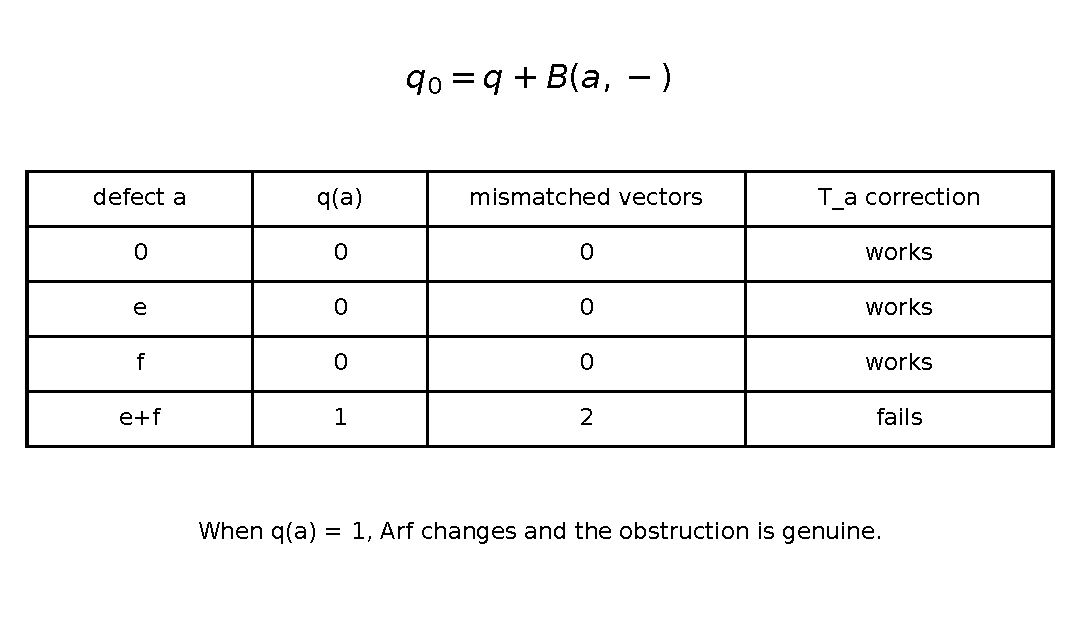
\includegraphics[width=\linewidth]{figures/V26.pdf}\end{center}
For the fixed hyperbolic plane $q=xy$, every refinement with the same polar form is $q_0=q+B(a,-)$ for one vector $a$. The table lists all four defect vectors. Its mismatch column counts the vectors at which $q_0(T_av)\ne q(v)$.
\[
q_0(T_av)=q(v)+B(a,v)q(a),\qquad
\operatorname{Arf}(q_0)+\operatorname{Arf}(q)=q(a).
\]
When $q(a)=0$, the correction works everywhere. For $a=e+f$, the Arf sign changes and two vectors still fail. This is not an unlucky choice of basis. In equal dimension, the two forms are not isometric.

In a larger host this test applies to the pullback along the supplied embedding. A different permitted subspace may behave differently. Under genuine supplied actions preserving both refinements and an initially equivariant embedding, the defect vector is fixed by the group. The same transvection is then equivariant. Those initial actions are hypotheses, not outputs of this linear solve.
\vfill\PlateSource{Exact defect enumeration}{Part III, Section 28}{71}
